\subsection{Theorie zur Ablenkung im elektrischen Feld}
Die Elektronen können nur nach Durchfliegen eines möglichst luftleeren Raum auf einem Schirm sichtbar gemacht werden, da sie sonst mit den Luftmolekülen zusammenstoßen.
\\Bewegen sich die Elektronen durch ein homogenes elektrisches Feld, zum Beispiel durch einen Kondensator, werden sie von diesem abgelenkt.
Die Ablenkung wird durch ein elektrisches Feld zwischen den Kondensatorplatten iniziiert.
Das negativ geladene Elektron wird gleichmäßig von der negativen Kondensatorplatte abgestoßen und von der positiv geladenen Platte angezogen.
Die Geschwindigkeit eines Elektrons in Richtung der Feldlinien, hier in Z-Richtung, lässt sich aus der angelegte Beschleunigungsspannung $U_{B}$ und der Energieerhaltung berechnen:
\begin{equation}
  E_{kin.}=E_{elektr.} \Leftrightarrow \frac{1}{2}m_{0}v_{Z}^{2}=e_{0}U_{B} \Leftrightarrow v_{Z}= \sqrt{ \frac{2 \: e_{0} \: U_{B}} {m_{0}} }.
\label{eqn:eerh}
\end{equation}
\\Dabei ist $m_{0}$ die Elektronenmasse und $e_{0}$ die Elementarladung.
\\Die Elektronen können auch eine Anfangsgeschwindigkeit senkrecht zu den Feldlinien haben.
Dies führt zu einer Ablenkung innerhalb des Kondensators analog zu einem waagerechten Wurf in der Mechanik.
Die parallel zum E-Feld wirkende Kraft führt zur Beschleunigung des Elektrons, hier in Y-Richtung:
\begin{equation*}
  F=e_{0}E=e_{0}\cdot \frac{U_{B}}{d}=m_{0}a_{Y} \Leftrightarrow a_{Y}= \frac{e_{0}\: U_{B}}{m_{0} \: d}.
\end{equation*}
\\Der Abstand der Kondensatorplatten ist durch $d$ beschrieben, die Länge der Kondensatorplatten ist $p$.
\\Aus der Beschleunigung der Elektronen lässt sich nun die Geschwindigkeit des Elektrons in Y-Richtung berechnen:
\begin{equation}
  v_{Y}=a \Delta t=\frac{e_{0}\:U_{B}}{m_{0}\:d}\cdot \Delta t
\label{eqn:vy}
\end{equation}
\\Die Geschwindigkeit des Elektronenstrahls in Z-Richtung im Kondensator ist konstant:
\begin{equation}
  \Delta t = \frac{p}{v_{Z}}.
\label{eqn:vz}
\end{equation}
\\Die Gleichungen \eqref{eqn:vy} und \eqref{eqn:vz} kombiniert ergeben die resultierende Geschwindigkeit in Y-Richtung in Abhängigkeit der Geschwindigkeit in Z-Richtung:
\begin{equation*}
  v_{Y}=a \Delta t=\frac{e_{0}\:U_{B}p}{m_{0}\:d \:v_{Z}}.
\end{equation*}
\\
\\Eine Möglichkeit der Darstellung eines abgelenkten Elektronenstrahls ist die Kathodenstrahlröhre.
In einer Kathodenstrahlröhre passiert der Elektronenstrahl mehrere ablenkende elektrische Felder und trifft dann auf einen Leuchtschirm.
Sobald der Elektronenstrahl das E-Feld verlässt, bewegt er sich linear weiter (Abb. \ref{fig:ablenkung}).
\begin{figure}[h!]
  \centering
  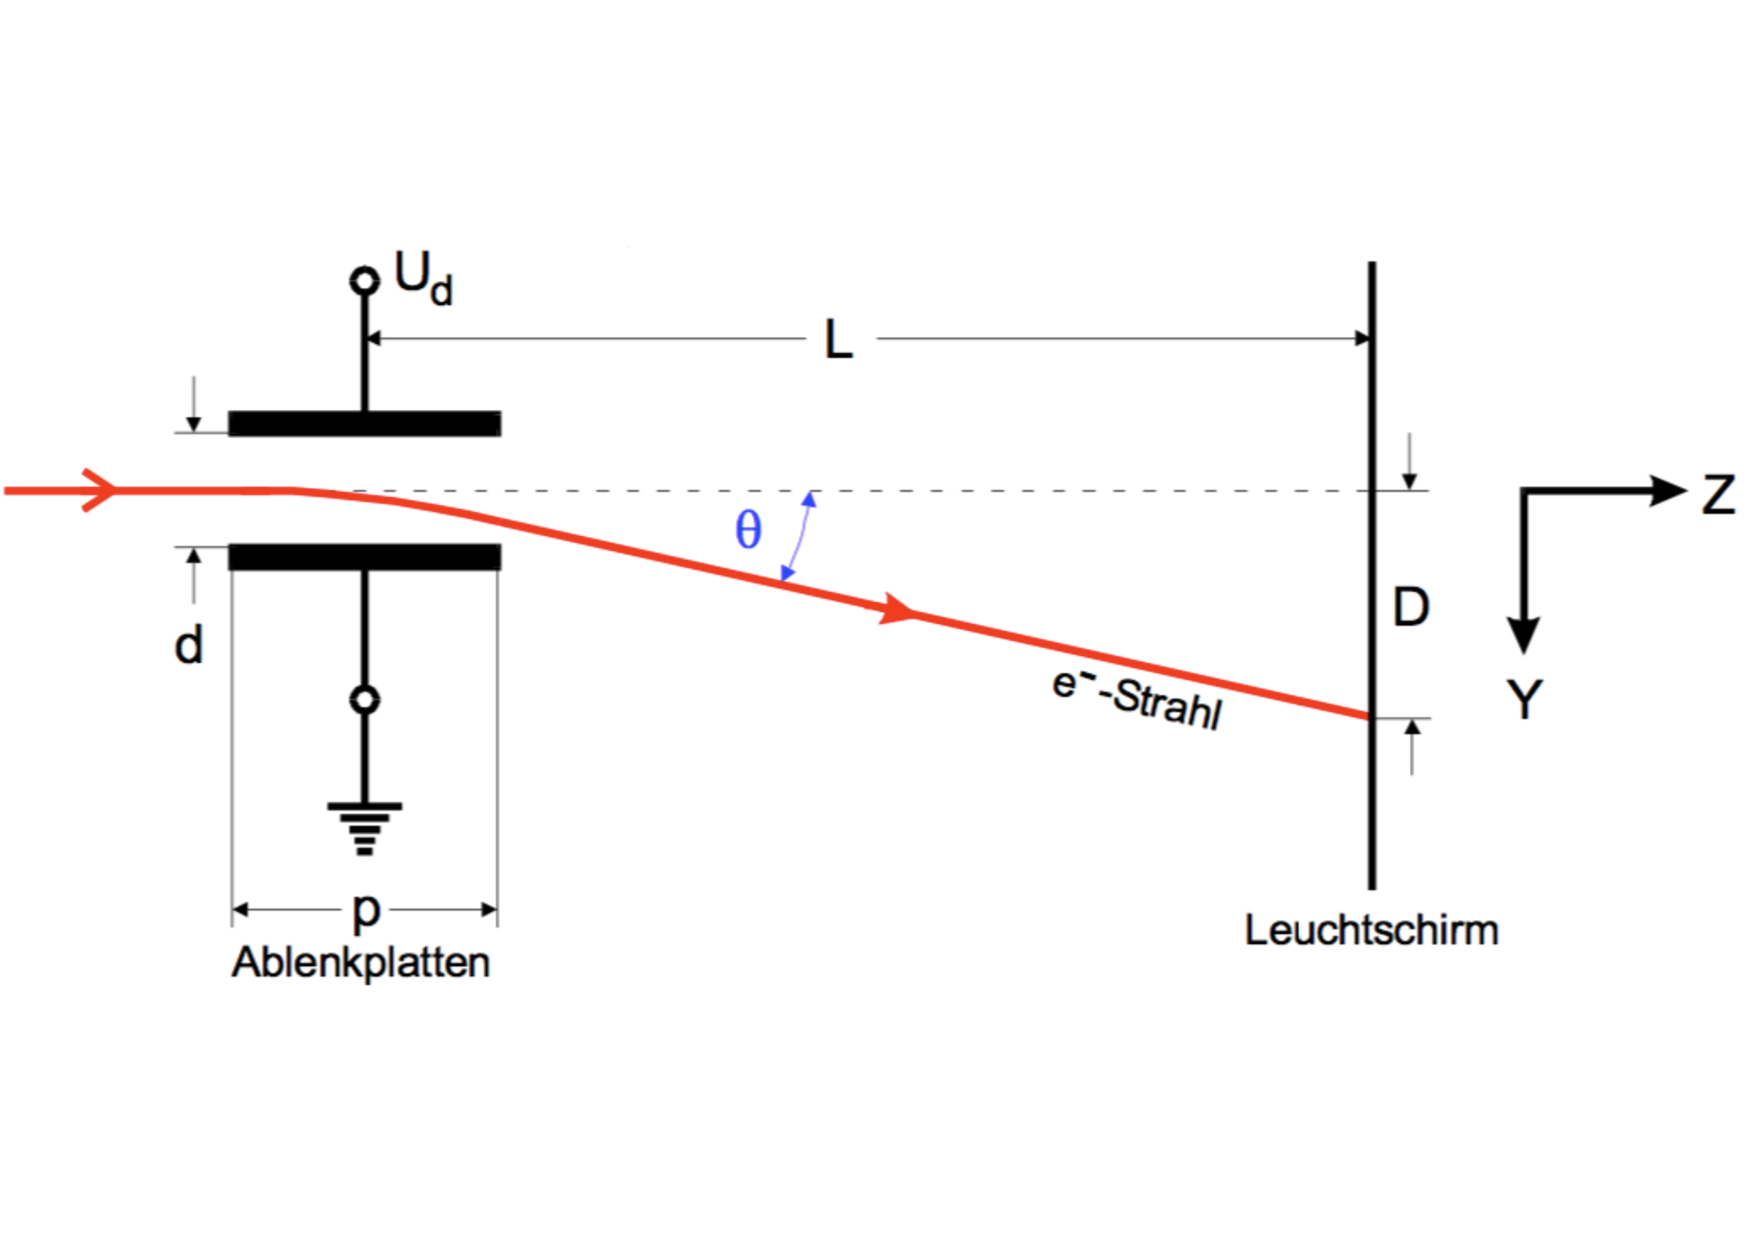
\includegraphics[width=0.8\textwidth]{EFeld2.pdf}
  \caption{Ablenkung des Elektronenstrahls durch die E-Felder \cite{1}}
  \label{fig:ablenkung}
\end{figure}
\\Der entsprechende Ablenkungswinkel $\theta$ ergibt sich durch:
\begin{equation*}
  \Theta = \frac{v_{Y}}{v_{Z}}=\frac{e_{0}\:U_{B}\:p}{m_{0}\:d \:v_{Z}^2}.
\end{equation*}
\\Der Abstand des Punktes zu seinem Ausgangspunkt berechnet sich wie folgt:
\begin{equation*}
  D= L \Theta = \frac{e_{0}\:U_{B}\:p \:L}{m_{0}\:d\: v_{Z}^2}.
\end{equation*}
\\L ist dabei der Abstand vom Kondensator bis zum Leuchtschirm.
\\Der zweite Ablenkungskondensator funktioniert analog. Er steht senkrecht zum ersten und ermöglicht ein zweidimensonales Bild auf dem Schirm.
Der Schirm besteht aus einem Material, welches bei Anregung durch Elektronen fluoresziert.
\\Die Kathodenstrahlröhre lässt sich als Oszilloskop, also zum Darstellen eines Spannungsverlaufes, verwenden.
Dazu wird an die Ablenkungsplatten in X-Richtung eine Sägezahnspannung der Frequenz $\nu_{säg}$ angelegt.
An die Ablenkplatten in Y-Richtung wird die Spannung gelegt, die untersucht werden soll mit der Frequenz $\nu_{sin}$.
Dabei müssen die Frequenzen beider Spannungen in einem richtigen Verhältnis stehen, um einen eindeutigen Spannungsverlauf darzustellen:
\begin{equation*}
  n\nu_{säg} = m\nu_{sin} \quad n=1,2,3,... \quad m=1,2,3,...
\end{equation*}
\FloatBarrier
\subsection{Theorie zur Ablenkung im magnetischen Feld}
Annähernd homogene Magnetfelder können durch ein Helmholtzspulenpaar erzeugt werden.
Der Betrag der magnetischen Flussdichte $B$ in der Mitte der Spulen berechnet sich durch:
\begin{equation}
B_{hor}=\frac{8 \: \mu_{0} \: N \: I }{\sqrt{125} \: R}.
\label{eqn:bhor}
\end{equation}
\\In einem homogenen magnetischen Feld wirkt die Lorentzkraft auf eine Ladung $q$ mit der Geschwindigkeit $v$:
\begin{equation*}
  \vec{F_{L}}=q\: \vec{v} \times \vec{B}
\label{eqn:lorentz}
\end{equation*}
\\Die Lorentzkraft führt zu einer Kreisbewegung der Ladung.
Dabei bleibt dennoch der Betrag der Geschwindigkeit konstant.
\\Zur Veranschaulichung der Lorentzkraft kann ein Elektronenstrahl mit einer Kathodenstrahlröhre erzeugt werden.
Im Bereich zwischen den Ablenkungskondensatoren und dem Leuchtschirm werden die Elektronen durch das B-Feld abgelenkt (Abb. \ref{fig:bfeld}).
\begin{figure}[h!]
  \centering
  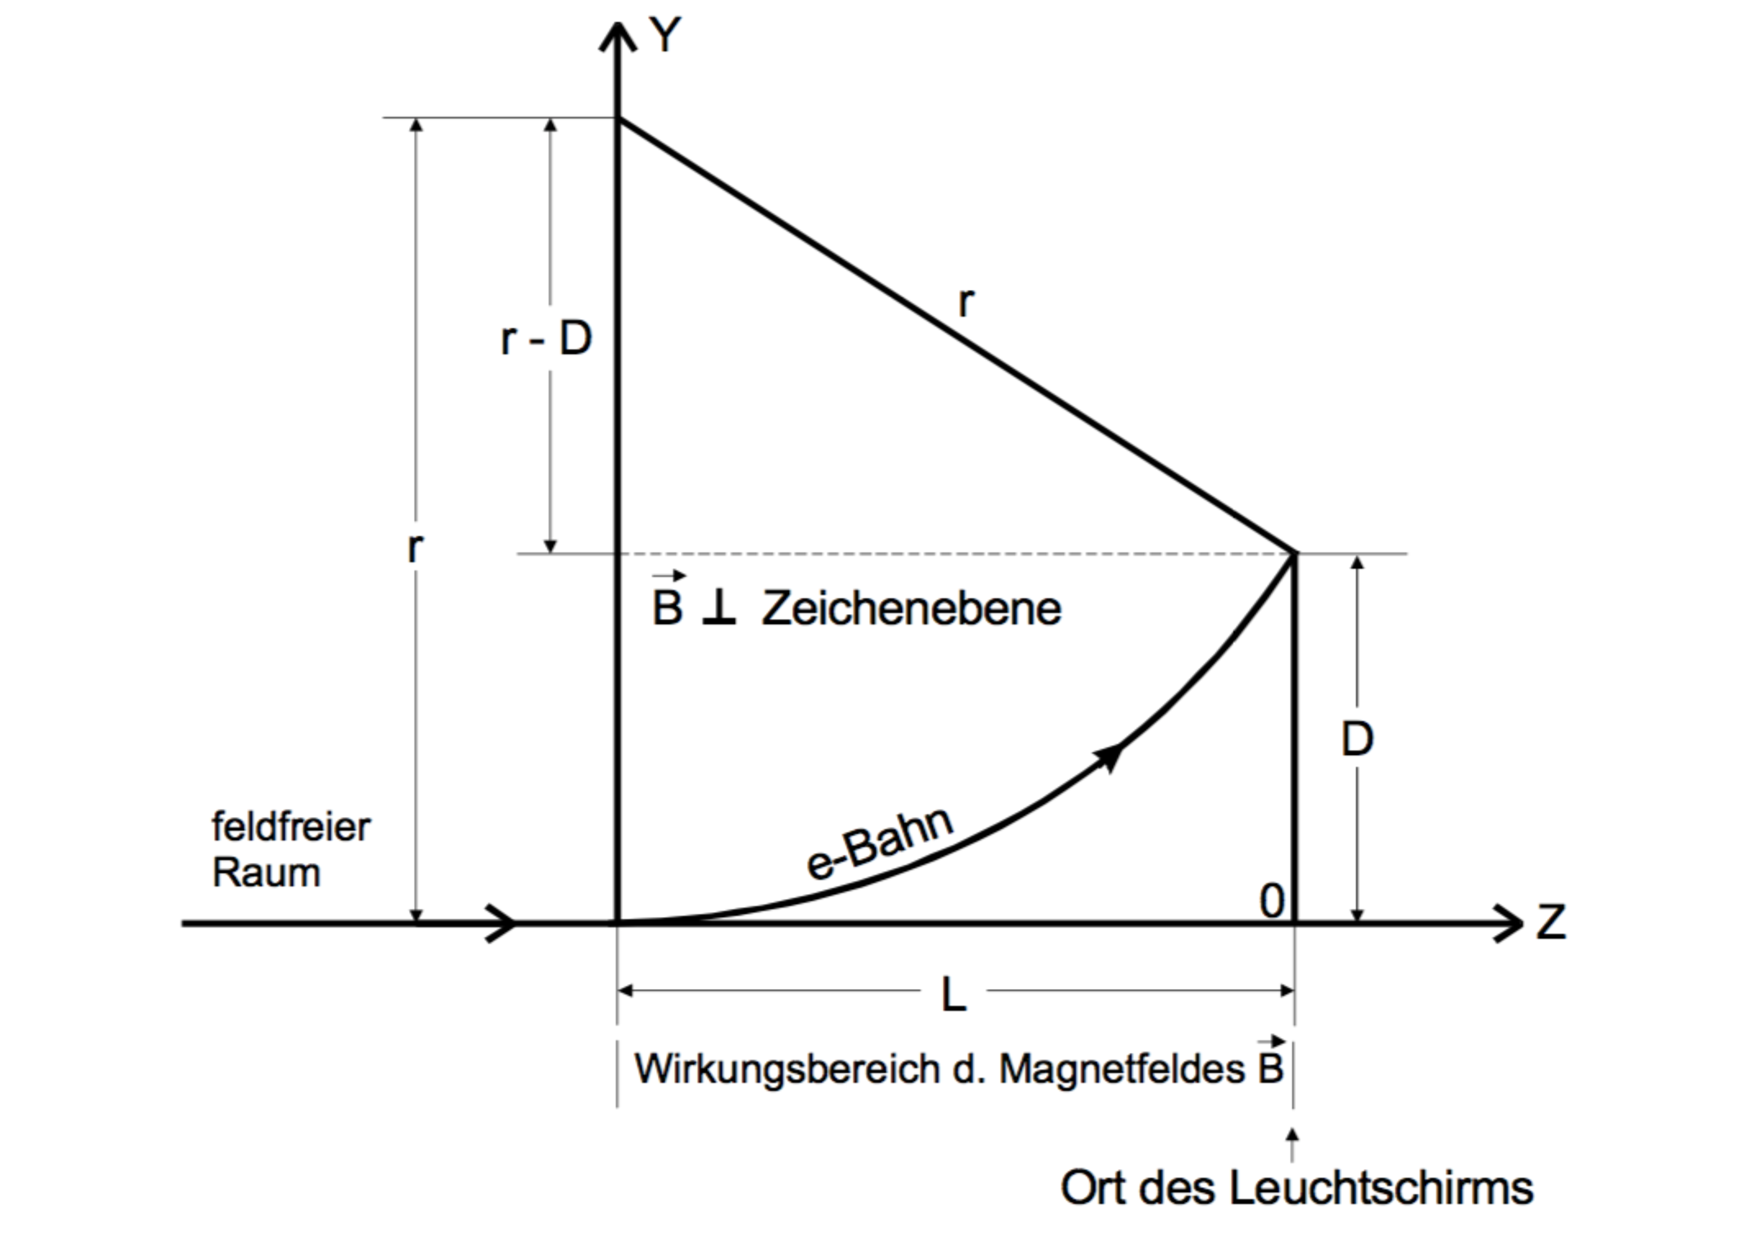
\includegraphics[width=0.8\textwidth]{Magnetfeld.pdf}
  \caption{Ablenkung des Elektronenstrahls durch das B-Feld \cite{2}}
  \label{fig:bfeld}
\end{figure}
\\Ist die Ladung die eines Elektrons und stehen die Bewegungsrichtung des Elektrons und die Richtung des B-Felds senkrecht aufeinander ergibt sich die Kraft zu:
\begin{equation*}
  F_{L}=e_{0} \: v \: B.
\end{equation*}
\\Die Zentripetalkraft ist im Gleichgewicht mit der Lorentzkraft:
\begin{equation*}
  F_{L}=F_{Z} \Leftrightarrow e_{0} v B = \frac{m_{0} v^2}{r}.
\end{equation*}
\\Dabei ist $r$ der Radius der Kreisbewegung, der sich ergibt zu:
\begin{equation}
  r=\frac{m_{0} \: v}{e_{0} \: B}
\label{eqn:rzentri}
\end{equation}
\\Um den Krümmungsradius durch die Höhe des Auftreffpunktes auf dem Schirm $D$ auszudrücken folgt durch den Satz des Pythagoras \ref{fig:bfeld}:
\begin{equation}
  L^2+(r-D)^2=r^2 \Leftrightarrow r= \frac{L^2+D^2}{2D}
\label{eqn:rkrümm}
\end{equation}
\\Aus Formel \eqref{eqn:rzentri}, Formel \eqref{eqn:rkrümm} und Formel \eqref{eqn:eerh} lässt sich schließen:
\begin{equation}
  \frac{m_{0} \: v}{e_{0} \: B} = \frac{L^2+D^2}{2D}
  \Leftrightarrow \sqrt{ \frac{m_{0}} {e_{0}}}=\frac{(L^2+D^2)B} {\sqrt{8 \: U_{B}} D}
  \Leftrightarrow \frac{e_{0}} {m_{0}}=\frac{8 \: U_{B} \: D^2} {(L^2+D^2)^2 \: B^2}
  \label{eqn:e0m0}
\end{equation}
\\Da die horizontal gemessene Feldstärke nicht der totalen Feldstärke entspricht, muss der Inklinationswinkel $\varphi$ noch einbezogen werden.
Die Feldlinien treten in unterschiedlichen Winkeln aus der Erdoberfläche (Abb. \ref{fig:erde}).
\begin{figure}[h!]
  \centering
  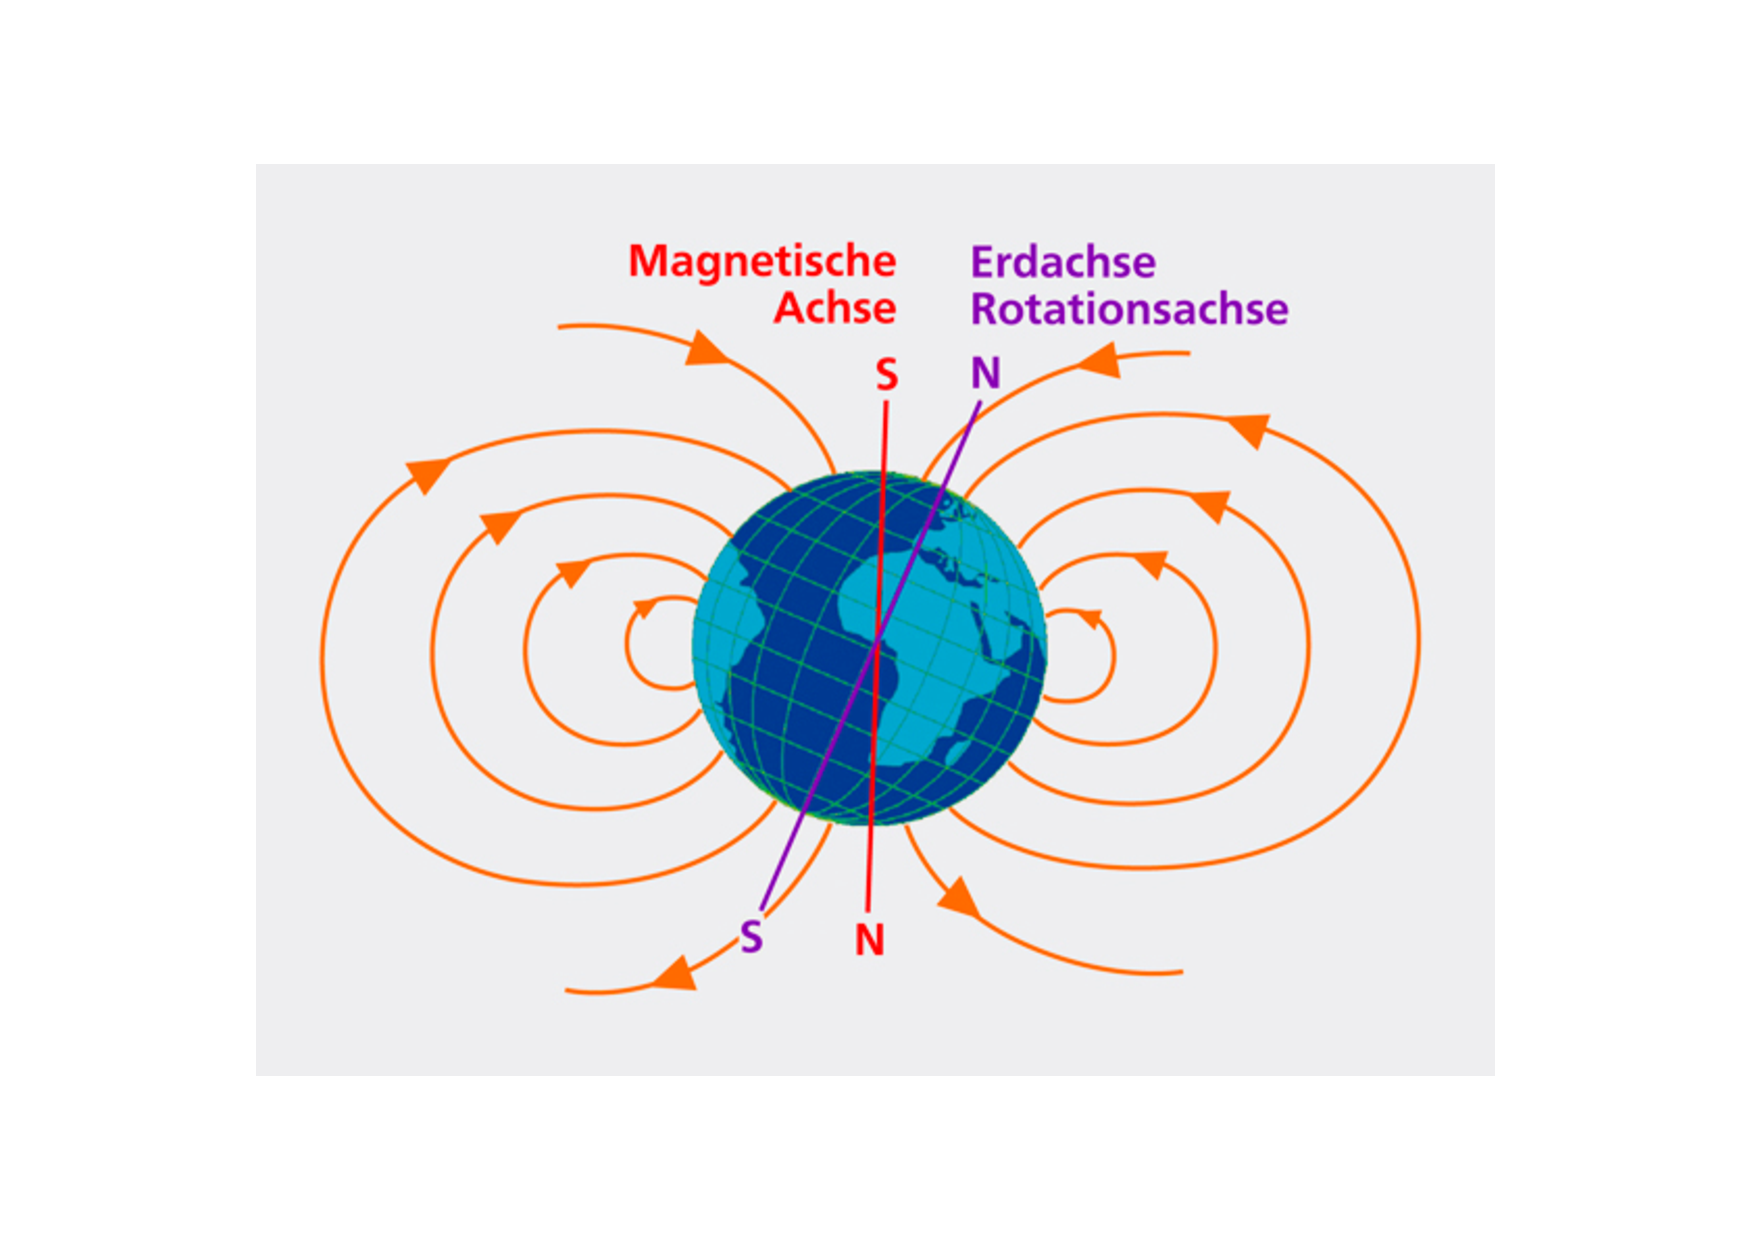
\includegraphics[width=0.8\textwidth]{erde.pdf}
  \caption{Feldlinien des Erdmagnetfelds \cite{3}}
  \label{fig:erde}
\end{figure}
\\Die totale Intensität des Erdmagnetfelds ergibt sich über die Winkelbeziehung zu
\begin{equation}
  B_{tot}=\frac{B_{hor}}{\cos{\varphi}}.
  \label{eqn:btot}
\end{equation}
\FloatBarrier
